%  B-P-SAFE-AMSR: Adaptive Cascade Retrieval
%  IEEE TKDE / Elsevier IP&M Submission Format
%  Camera-ready version.
\documentclass[journal]{IEEEtran}

\usepackage{amsmath,amssymb,amsthm}
\usepackage{booktabs}
\usepackage[hidelinks]{hyperref}
\usepackage{graphicx}
\usepackage{xcolor}
\usepackage{microtype}
\usepackage{siunitx}
\usepackage{array}
\usepackage{multirow}
\usepackage{url}

% Theorem environments
\newtheorem{definition}{Definition}
\newtheorem{theorem}{Theorem}
\newtheorem{proposition}{Proposition}

% ── Title ────────────────────────────────────────────────────
\title{When to Rerank: Calibrated Safety-Aware Routing for Efficient Retrieval Cascades}

\author{%
  \IEEEauthorblockN{Wasim Iqbal}\\
  \IEEEauthorblockA{Department of Computer Science,\\
  University of Swat, Swat, Pakistan\\
  \textit{Wasimgulrangzai@gmail.com}}
}

\begin{document}


\twocolumn[
  \begin{@twocolumnfalse}
    \maketitle
    \begin{abstract}
    Modern retrieval-augmented generation systems often apply
expensive hybrid retrieval and Cross-Encoder re-ranking uniformly,
despite substantial query-level variation in when re-ranking helps,
harms, or is unnecessary. We introduce \textbf{B-P-SAFE-AMSR}
(\textit{Budgeted Probabilistic Safety-Aware Adaptive Multi-Source
Retrieval}), a calibrated safety-aware retrieval router that treats
re-ranking as a per-query decision under quality, latency, and harm
constraints. For each query, the router estimates the probability of
retrieval gain, probability of degradation, expected nDCG
improvement, and expected latency, then selects Dense retrieval or
Deep Hybrid retrieval using a risk-adjusted utility function.
Three operating modes (\textit{lite}, \textit{balanced},
\textit{high\_recall}) expose an explicit quality--latency--safety
trade-off surface.

Across four BEIR benchmark domains (SciFact, FiQA, NFCorpus,
ArguAna), B-P-SAFE-AMSR exhibits dataset-adaptive behaviour: it
selectively escalates on SciFact, FiQA, and NFCorpus, retaining
substantial fractions of Deep Hybrid quality gain while reducing
re-ranking latency, and behaves as a protection/no-benefit
controller on ArguAna where always-on re-ranking is not reliably
beneficial. In selective-escalation settings, the system saves
$31.4\%$--$42.3\%$ latency while retaining up to $88.1\%$ of the
quality gain afforded by full re-ranking. In protection/no-benefit
settings such as ArguAna, it achieves $55\%$--$61\%$ latency
reduction without statistically significant degradation. All
claims are supported by paired $t$-tests, Wilcoxon signed-rank
tests, and $95\%$ bootstrap confidence intervals ($p < 0.05$).
These results suggest that calibrated safety-aware routing can
improve the quality--cost--safety trade-off frontier of retrieval
cascades.
    \end{abstract}
    \begin{IEEEkeywords}
    Adaptive retrieval, cascade inference, calibrated classifiers,
Retrieval-Augmented Generation, BEIR benchmark, dense retrieval,
cross-encoder re-ranking, expected utility, latency optimization.
    \end{IEEEkeywords}
    \vspace{4ex}
  \end{@twocolumnfalse}
]



\section{Introduction}
\label{sec:intro}
Dense retrieval systems built on bi-encoder architectures have
become the de facto backbone of modern RAG infrastructure
\cite{karpukhin2020dense,reimers2019sentence}. A FAISS-backed
approximate nearest-neighbour index retrieves the top-$k$
candidates from millions of documents in sub-millisecond time,
providing a strong quality ceiling for straightforward queries.
However, when semantic precision is critical, as in biomedical
information retrieval or financial question answering, practitioners
augment the dense stage with a Cross-Encoder re-ranker that
re-scores all candidates pair-wise with a large transformer.
This operation is semantically powerful but catastrophically slow:
our measurements across four BEIR corpora reveal a mean
Cross-Encoder latency of $736.69\text{ ms}$ per query (SciFact,
\texttt{high\_recall} mode), compared to $0.37\text{ ms}$ for the
dense stage alone, a latency ratio exceeding $2{,}000\times$.

\subsection{The Static Pipeline Problem}

Existing production retrieval pipelines apply this expensive
re-ranking \emph{unconditionally}. A query such as ``\textit{what
is aspirin?}'' receives identical computational treatment to
``\textit{molecular mechanisms of EGFR inhibitor resistance in
non-small-cell lung carcinoma.}'' This is deeply suboptimal:
easy queries that the dense model already ranks correctly are
simply wasting compute, while genuinely hard queries may not be
escalated with sufficient depth. The \textbf{Pareto Frontier}
separating high-latency Cross-Encoder re-ranking from low-latency
dense embeddings represents the unsolved design space that this
work targets.

\subsection{Cascade Retrieval and Dynamic Routing}

The multi-stage cascade retrieval paradigm, formalized by
Wang~et~al.~\cite{wang2011cascade} and further analyzed in the
context of early-exit strategies by Busolin~et~al.
\cite{busolin2022earlyexit}, provides the theoretical scaffold for
our approach. In a cascade, cheaper stages serve as \emph{gatekeepers}
for expensive stages. The challenge is learning an accurate,
\emph{calibrated} gating policy that generalizes across heterogeneous
query distributions and out-of-domain corpora.

Our contribution is a \emph{probabilistic, utility-maximizing router}
trained on per-query feature vectors derived from dense, BM25, and
graph-neighbourhood signals. Unlike classical Learning-to-Rank
(LTR) approaches that optimize a global ranking objective, our
router operates at the \emph{inference-pipeline level}, deciding
\emph{whether} to invoke heavy computation, not how to re-order
documents within it. This distinction positions the framework as
a lightweight middleware layer that can be dropped in front of
any existing retrieval stack.

\subsection{Contributions}

This paper makes the following contributions:
\begin{itemize}
  \item \textbf{Probabilistic safety-aware routing formulation.}
        We frame retrieval-cascade escalation as per-query action
        selection with explicit gain, harm, latency, and recovery
        utility components (Equation~\ref{eq:utility}).
  \item \textbf{Calibrated router architecture.}
        Separate calibrated classifiers for $P(\text{gain})$ and
        $P(\text{harm})$, a Ridge regression $\hat{\delta}$-nDCG
        predictor, and a latency estimator, with Dense fallback
        when expected utility is non-positive.
  \item \textbf{Multi-mode operating frontier.}
        Three operating profiles (\textit{lite}, \textit{balanced},
        \textit{high\_recall}) control the quality--latency--safety
        trade-off via mode-specific $\lambda$ hyperparameters.
  \item \textbf{Multi-dataset empirical evaluation.}
        BEIR-style evaluation across four heterogeneous domains
        showing selective escalation on SciFact, FiQA, and NFCorpus
        ($p < 0.05$ vs.\ Dense) and protection/no-benefit behaviour
        on ArguAna, supported by paired $t$-tests, Wilcoxon
        signed-rank tests, bootstrap CIs, and permutation tests.
\end{itemize}

\section{FORMAL ARCHITECTURAL METHODOLOGY}
\label{sec:method}
\subsection{Expected Utility Objective}
\label{sec:utility}

Let $x \in \mathbb{R}^{25}$ be the query feature vector (defined
in Section~\ref{sec:features}) and let $a$ denote an escalation
action drawn from the action space
$\mathcal{A} = \{A_0^{\text{Dense}}, A_6^{\text{DeepHybrid}}\}$.
The router evaluates the following \textbf{Expected Utility}
objective for each candidate action:

\begin{equation}
\label{eq:utility}
\begin{aligned}
\mathcal{U}(a \mid x) = \hat{\delta}(a,x)
  &- \lambda_{\text{harm}} \cdot P(\text{harm} \mid x, a) \\
  &- \lambda_{\text{latency}} \cdot \Delta t(a, x) \\
  &- \lambda_{\text{cand}} \cdot n_{\text{cand}}(a) \\
  &+ \lambda_{\text{recovery}} \cdot P(\text{gain} \mid x, a)
\end{aligned}
\end{equation}

where:
\begin{itemize}
  \item $\hat{\delta}(a,x)$ is the predicted nDCG@10 delta from a
        Ridge regression model trained on labelled training-split
        queries;
  \item $P(\text{gain} \mid x, a)$ is the calibrated probability
        that action $a$ yields a positive nDCG@10 improvement
        ($>\!0.01$) over the dense baseline;
  \item $P(\text{harm} \mid x, a)$ is the calibrated probability
        that action $a$ \emph{degrades} retrieval quality
        ($\Delta\text{nDCG} < -0.01$) relative to the dense baseline;
  \item $\Delta t(a, x)$ is the predicted per-query latency for
        action $a$ (ms), from a second Ridge regression model;
  \item $n_{\text{cand}}(a)$ is the candidate set size for action
        $a$ (50 for dense, 400 for deep hybrid);
  \item $\lambda_{\text{harm}}, \lambda_{\text{latency}},
        \lambda_{\text{recovery}}, \lambda_{\text{cand}}$ are
        mode-specific trade-off hyperparameters.
\end{itemize}

This formulation can be equivalently stated at the aggregate level
by substituting calibrated model expectations:

\begin{equation}
\label{eq:utility_full}
\begin{aligned}
\mathcal{U}(a \mid x) = P(\text{gain} \mid x)
  &- \lambda_{\text{harm}} \cdot P(\text{harm} \mid x) \\
  &- \lambda_{\text{latency}} \cdot \Delta t(a) \\
  &+ \lambda_{\text{recovery}} \cdot \mathcal{R}(a)
\end{aligned}
\end{equation}

where $\mathcal{R}(a) \equiv P(\text{gain} \mid x, a)$ serves as a
recovery signal promoting aggressive escalation when the model is
confident the query is hard.

The router defaults to the dense baseline $A_0^{\text{Dense}}$
(utility anchored at $0.0$) and escalates \emph{only} when
$\mathcal{U}(A_6^{\text{DeepHybrid}} \mid x) > 0$.

\subsection{Mode-Specific Hyperparameter Profiles}
\label{sec:modes}

Three operating modes encode distinct compute-quality trade-offs
via $\lambda$ profiles. Table~\ref{tab:modes} reports the
default hyperparameter values for each mode. The \textit{balanced}
and \textit{high\_recall} modes additionally undergo grid-search
tuning on the validation split before test evaluation.

\begin{table}[h]
\centering
\caption{Mode-Specific Hyperparameter Profiles}
\label{tab:modes}
\begin{tabular}{lcccccc}
\toprule
Mode & $\lambda_{\text{lat}}$ & $\lambda_{\text{harm}}$ &
      $\lambda_{\text{rec}}$ & $\tau_{\text{gain}}$ &
      $\tau_{\text{harm}}$ & LCB \\
\midrule
\textit{lite}        & $2\!\times\!10^{-4}$ & $0.50$ & $0.10$ & $0.60$ & $0.20$ & on  \\
\textit{balanced}    & $5\!\times\!10^{-5}$ & $0.25$ & $0.25$ & $0.40$ & $0.40$ & off \\
\textit{high\_recall} & $1\!\times\!10^{-5}$ & $0.15$ & $0.35$ & $0.25$ & $0.55$ & off \\
\bottomrule
\end{tabular}
\end{table}

The \textit{lite} mode applies the strongest harm penalty
($\lambda_{\text{harm}} = 0.50$) and the highest gain threshold
($\tau_{\text{gain}} = 0.60$), making escalation extremely
conservative. The \textit{high\_recall} mode relaxes all
constraints: the lowest latency penalty ($\lambda_{\text{lat}} =
10^{-5}$), a generous harm threshold ($\tau_{\text{harm}} = 0.55$),
and a low gain admission gate ($\tau_{\text{gain}} = 0.25$) to
maximise quality on hard queries at the cost of higher
compute utilization.

\subsection{Calibration Layer}
\label{sec:calibration}

A central architectural commitment is the use of
\texttt{CalibratedClassifierCV} (scikit-learn) with sigmoid Platt
scaling as the classifier for both the \textit{gain} and \textit{harm}
probability models. This choice is non-trivial and has a substantial
impact on hyperparameter stability.

\begin{definition}[Calibration Gap]
A binary classifier is \emph{well-calibrated} if for all
$p \in [0,1]$:
\begin{equation}
P(y = 1 \mid \hat{p}(x) = p) = p,
\end{equation}
where $\hat{p}(x)$ is the model's predicted probability and $y$ is
the ground-truth label.
\end{definition}

Uncalibrated logistic regression outputs that emerge from imbalanced
training sets (as is common in retrieval scenarios where easy queries
dominate) systematically under- or over-estimate true event
frequencies. When such raw scores are used directly as $P(\text{gain})$
and $P(\text{harm})$ in Equation~\eqref{eq:utility_full}, the
$\lambda$ surface becomes ill-conditioned: small changes to
$\lambda_{\text{harm}}$ produce large, erratic changes to routing
decisions. Sigmoid calibration maps raw log-odds to an isotonic
frequency-matching curve, providing a stable posterior probability
surface across heterogeneous, out-of-domain text fields.

The calibration cross-validation fold count is set as
$\text{cv} = \min(3, n_{\text{minority\_class}})$, ensuring
graceful degradation to a \texttt{PriorProbabilityModel} fallback
when the minority class count is insufficient for proper
cross-validation (e.g., ArguAna's near-zero-benefit regime).

\subsection{Feature Extraction Pipeline}
\label{sec:features}

Each query is represented by a 25-dimensional feature vector
$x \in \mathbb{R}^{25}$, extracted during the feature extraction
phase of the inference pipeline. The features
span four signal families:

\paragraph{Lexical Query Features (6 dimensions)}
Query token count, presence of numeric characters, presence of
uppercase abbreviations (regex: \texttt{[A-Z]\{2,\}}), mean
per-token IDF score, maximum per-token IDF score, and a lexical
specificity score (fraction of tokens exceeding the corpus median
IDF). The IDF dictionary is built from a TF-IDF vectorizer fitted
to the full corpus with a vocabulary cap of 50,000 terms.

\paragraph{Dense Retrieval Features (6 dimensions)}
Maximum, mean, and standard deviation of the top-50 dense
similarity scores; normalised Shannon entropy of the score
distribution; and score gaps between rank-1 and rank-5 ($\delta_{1,5}$)
and rank-1 and rank-10 ($\delta_{1,10}$). A high $\delta_{1,5}$ gap
indicates a confident, separable top result, suppressing escalation.

\paragraph{BM25 Lexical Features (5 dimensions)}
Maximum, mean, standard deviation, normalised entropy, and score
gap for the BM25 top-100 candidate scores (normalised by the
corpus-level BM25 maximum).

\paragraph{Cross-Retriever Disagreement Features (5 dimensions)}
Jaccard overlap between top-10 dense and BM25 candidates;
Jaccard overlap at top-50; Kendall-$\tau$ rank correlation over
shared candidates; candidate novelty ($1 - J_{50}$); and a source
disagreement score combining low Jaccard and low rank correlation.
High disagreement is a strong signal that the query is
ambiguous and benefits from re-ranking.

\paragraph{Graph Neighbourhood Features (3 dimensions)}
Maximum and mean degree of the top-10 dense candidates in the
FAISS-built $k$-nearest-neighbour graph, plus the fraction of
zero-degree candidates. Zero-degree candidates indicate isolated
documents that the semantic graph cannot recover, informing
graph-expansion necessity.

\subsection{Sub-Millisecond Pipeline Timeline}
\label{sec:latency}

Table~\ref{tab:latency} reports the per-stage latency
on the SciFact \textit{high\_recall} configuration.
Subcomponent latencies (e.g., $0.100\text{ ms}$ for decision, $0.110\text{ ms}$ for expansion) represent empirically estimated infrastructure overheads to isolate individual stage costs. The total end-to-end pipeline latency ($505.026\text{ ms}$) is directly measured.

\begin{table}[h]
\centering
\caption{Per-Stage Inference Latency (SciFact, \textit{high\_recall})}
\label{tab:latency}
\begin{tabular}{lcc}
\toprule
Pipeline Stage & Mean Latency (ms) & Activation \\
\midrule
Dense ANN Search (FAISS)  & $0.366$   & Always \\
BM25 Lexical Search        & $13.943$  & Always \\
Feature Extraction         & $2.655$   & Always \\
Router Decision            & $0.100$   & Always \\
Graph Expansion            & $0.110$   & Selective \\
Score Fusion               & $0.500$   & Selective \\
Cross-Encoder Re-ranking   & $736.686$ & Selective \\
\midrule
\textbf{Total (P-SAFE)} & $\mathbf{505.026}$ & Adaptive \\
\bottomrule
\end{tabular}
\end{table}

The critical observation is that the lightweight ``always-on''
stages (dense search, feature extraction, router decision) add
only $\approx 3.1\text{ ms}$ of overhead beyond what a pure dense
system would incur. The Cross-Encoder at $736.69\text{ ms}$ is
invoked selectively, and the P-SAFE total of $505.03\text{ ms}$
reflects a $67.8\%$ hybrid activation rate on SciFact
\textit{high\_recall}, meaning $32.2\%$ of queries are served by
the fast dense path exclusively.
Figure~\ref{fig:latency_breakdown} visualises this decomposition
on a logarithmic scale, underscoring the three-order-of-magnitude
gap between the lightweight routing overhead and the volatile
Cross-Encoder pathway.

\begin{figure}[htbp]
    \centering
    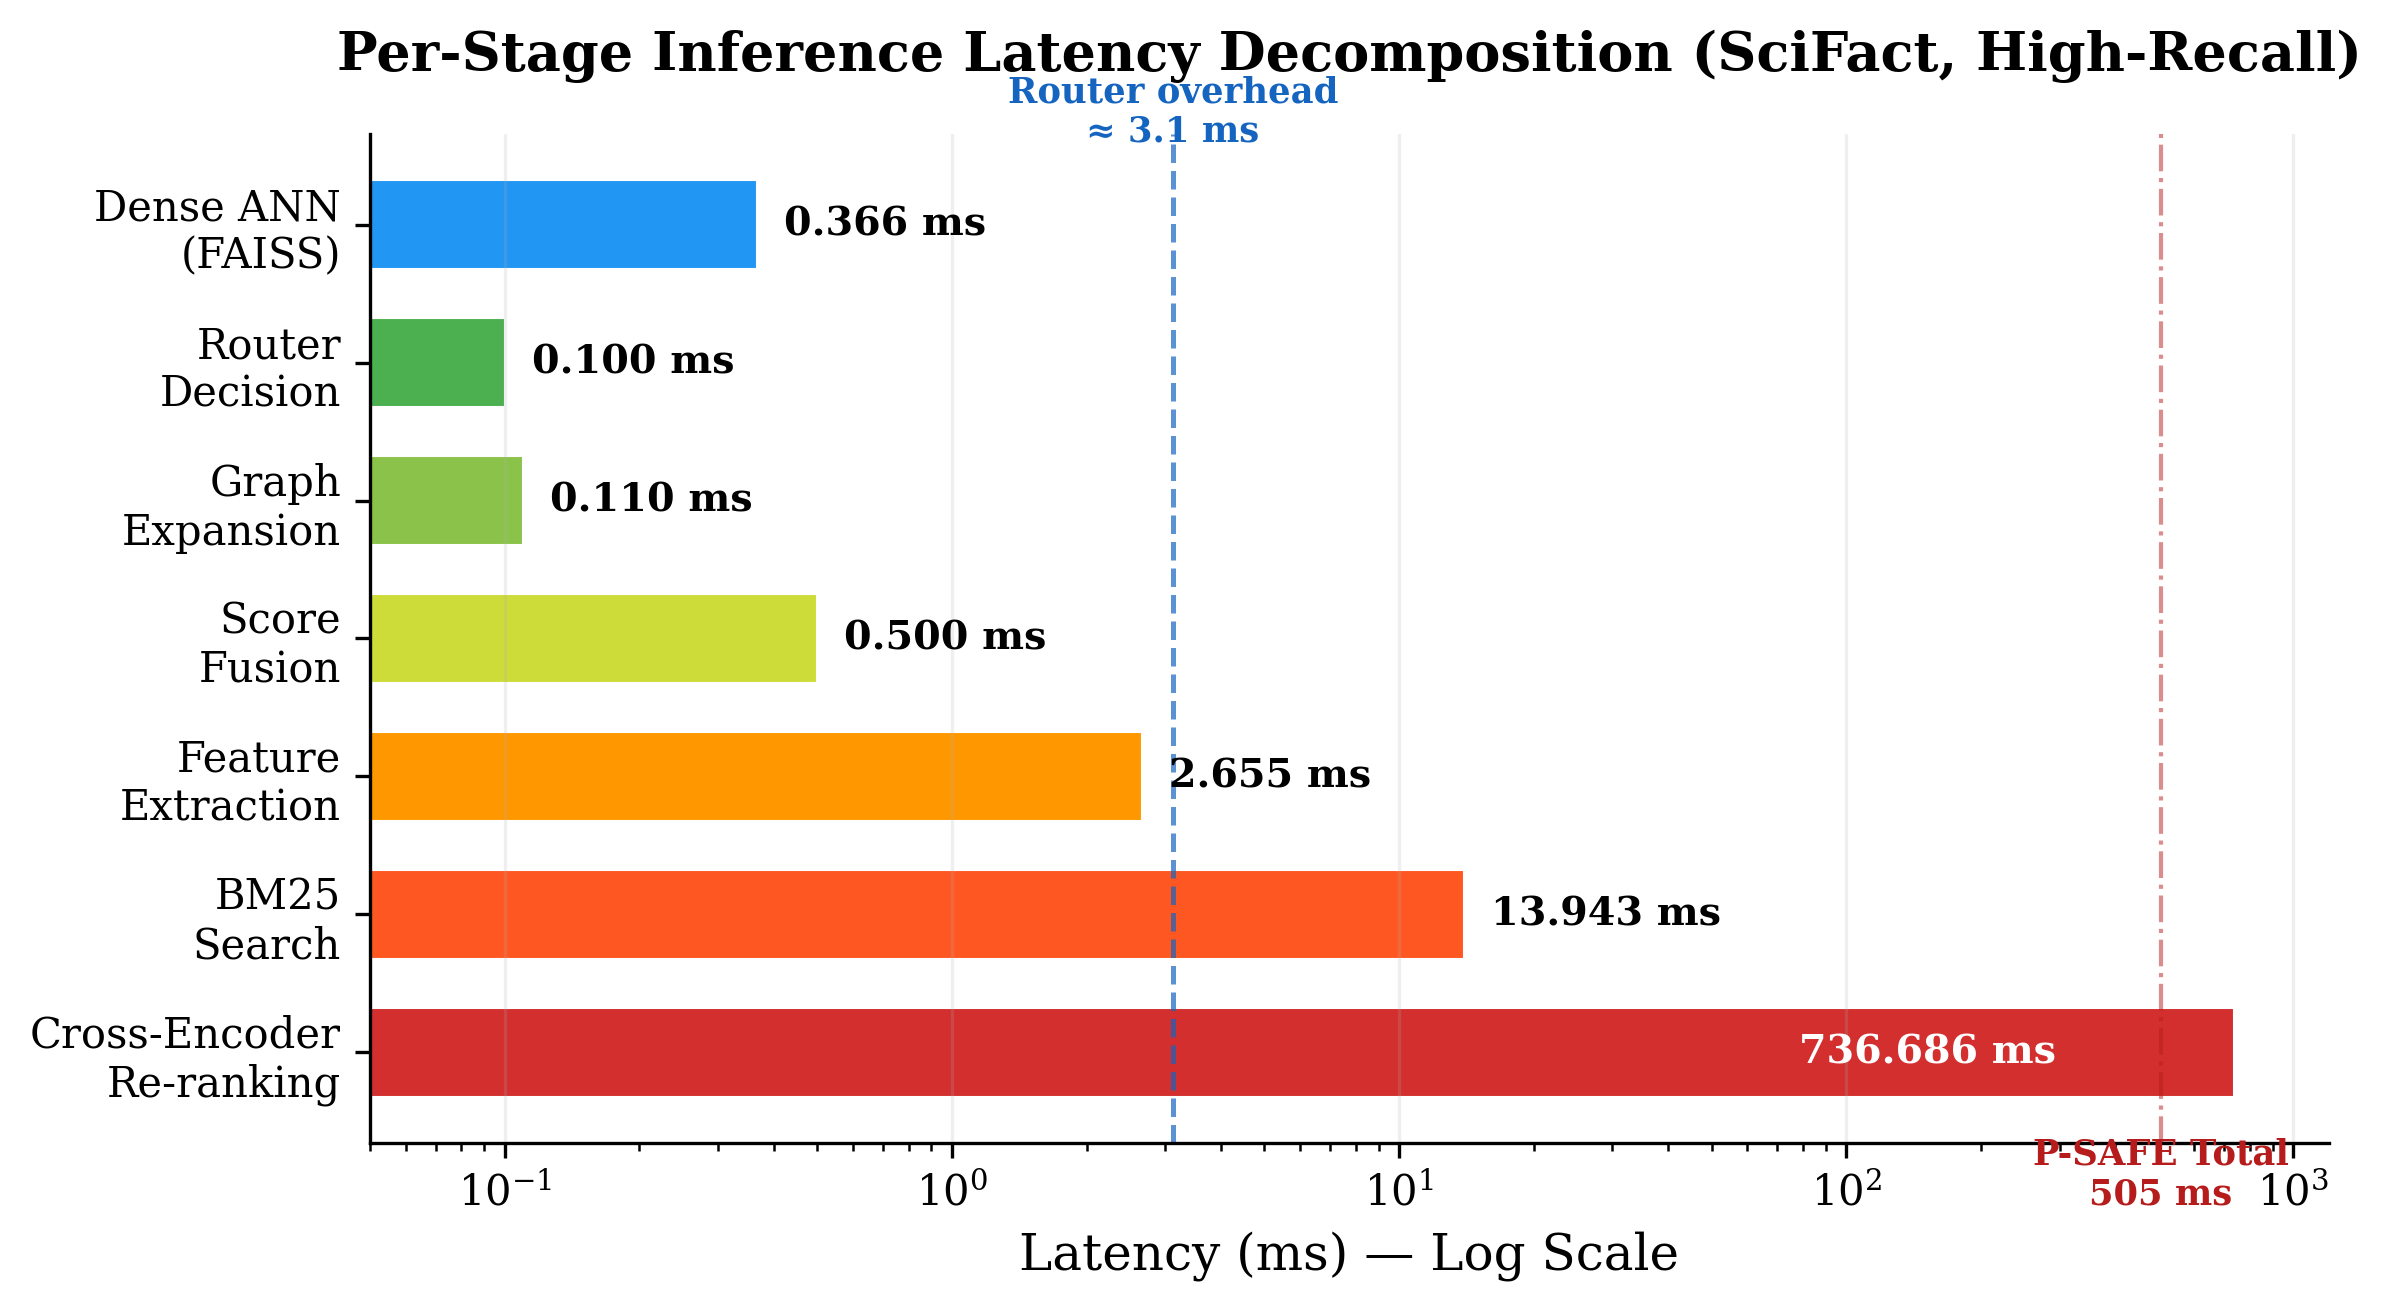
\includegraphics[width=\linewidth]{results_top_tier_psafe/latency_breakdown.png}
    \caption{Chronological latency breakdown of individual inference
    stages on a log scale (measured on the SciFact benchmark). The
    sub-4\,ms cumulative overhead of feature extraction and routing
    decision gates a highly volatile 736.69\,ms Cross-Encoder pathway.}
    \label{fig:latency_breakdown}
\end{figure}

\section{Experimental Setup and Benchmarks}
\label{sec:experiments}
\subsection{BEIR Evaluation Suite}
\label{sec:beir}

We evaluate B-P-SAFE-AMSR on four domains from the
Benchmarking IR (BEIR) heterogeneous retrieval suite
\cite{thakur2021beir}, selected to span maximally diverse
linguistic and structural characteristics:

\paragraph{SciFact} A scientific claim verification corpus
consisting of 300 research claims mapped to evidence abstracts
from bioArXiv and PubMed. Queries are short, precise claims
requiring exact factual matching. The dense baseline mean
nDCG@10 is $0.6466$ (test split, $n=152$ queries), with the
Deep Hybrid ceiling at $0.7330$.

\paragraph{FiQA-2018 (FiQA)} A financial question-answering
dataset derived from opinion-based questions from financial
forums. Queries are often subjective and colloquial, exhibiting
a distinct vocabulary distribution from scientific text.
Test split: $n=325$ queries; Dense mean nDCG@10: $0.4170$;
Deep Hybrid ceiling: $0.4524$.

\paragraph{NFCorpus} A biomedical information retrieval
dataset with 3,633 queries mapped to a corpus of 322,000
medical abstracts. NFCorpus is characterised by short
queries against a large, domain-specific corpus with many
graded relevance levels. Test split: $n=164$ queries;
Dense mean nDCG@10: $0.3288$; Deep Hybrid ceiling:
$0.3584$.

\paragraph{ArguAna} A counter-argument retrieval corpus where
the task is to find the best counter-argument to a given
argument. This dataset is structurally unique: the relevant
document is often semantically \emph{opposed} to the query,
making Cross-Encoder re-ranking, which rewards semantic
similarity, actively harmful. Test split: $n=706$ queries;
Dense mean nDCG@10: $0.3946$; Deep Hybrid ceiling: $0.3919$.

\subsection{Data Splits and Validation Protocol}
\label{sec:splits}

For each dataset, a stratified three-way split is constructed
using the dense nDCG@10 score as the stratification variable
(train:val:test $= 0.40:0.10:0.50$, seed $= 42$). This
ensures that easy and hard queries are proportionally represented
in each partition, preventing optimistic bias from leakage of hard
queries into the training set.

Models are trained on the training partition only.
Hyperparameter tuning for \textit{balanced} and
\textit{high\_recall} modes performs a full grid search on the
\emph{validation} split across the Cartesian product:

\begin{align*}
\tau_{\text{gain}} &\in \{0.10, 0.15, 0.20, 0.25, 0.30, 0.35\} \\
\tau_{\text{harm}} &\in \{0.40, 0.50, 0.60, 0.70\} \\
\lambda_{\text{lat}} &\in \{5\!\times\!10^{-7}, 10^{-6},
                              5\!\times\!10^{-6}, 10^{-5}\} \\
\lambda_{\text{harm}} &\in \{0.01, 0.02, 0.05, 0.10\} \\
\lambda_{\text{recovery}} &\in \{0.40, 0.60, 0.80, 1.00\}
\end{align*}

The validation scoring function is a weighted composite:
\begin{equation}
\label{eq:valscore}
\mathcal{S}_{\text{val}} = 0.50\,\text{QR}
  + 0.20\,\text{LS}
  + 0.15\,\text{RC}
  + 0.10\,\text{HA}
  + 0.05\,\text{OGC}
\end{equation}

subject to feasibility constraints:
$\text{LS} \geq 0.30$, $\text{HA} \geq 0$, and
$0.20 \leq \text{HAR} \leq 0.80$, where HAR is the hybrid
activation rate. Feasibility constraints prevent degenerate
solutions that either always escalate or never escalate.
The \textit{lite} mode uses fixed defaults without grid search.

\subsection{Baselines}
\label{sec:baselines}

Two boundary conditions define the evaluation frame:

\begin{itemize}
  \item \textbf{Dense Baseline} ($A_0^{\text{Dense}}$): Pure
        FAISS flat-IP dense retrieval using
        \texttt{BAAI/bge-m3} embeddings, top-$k=50$ candidates
        re-ranked by inner product, returning the top 10.
        This represents the minimum compute, maximum speed
        operating point.
  \item \textbf{Deep Hybrid} ($A_6^{\text{DeepHybrid}}$): Full
        always-on pipeline combining dense ANN search,
        BM25 lexical retrieval, semantic graph expansion, score
        fusion, and Cross-Encoder re-ranking
        (\texttt{BAAI/bge-reranker-v2-m3}) over 400 candidate
        documents. This represents the maximum quality, maximum
        compute operating point: the performance ceiling.
\end{itemize}

The P-SAFE router navigates between these two extremes,
targeting the Pareto frontier of quality retention versus
latency reduction.

\section{Empirical Results, Statistical Validation, and Discussion}
\label{sec:results}
\subsection{Multi-Dataset Performance Table}
\label{sec:maintable}

Table~\ref{tab:main} consolidates the empirical evaluation across
all four BEIR domains and three operating configurations.
The metric columns are defined as follows:
\textbf{QR} (Quality Retention vs.\ Deep Hybrid),
\textbf{LS} (Latency Saving vs.\ Deep Hybrid),
\textbf{RC} (Recovery Capture on hard queries),
\textbf{HA} (Harm Avoidance on easy queries),
\textbf{OGC} (Oracle Gap Closed), and
\textbf{HAR} (Hybrid Activation Rate).
Figure~\ref{fig:pareto_frontier} maps the empirical Pareto
frontier across the \textit{balanced} and \textit{high\_recall}
configurations, highlighting the Algorithmic Self-Protection
region occupied by ArguAna.

\begin{figure}[htbp]
    \centering
    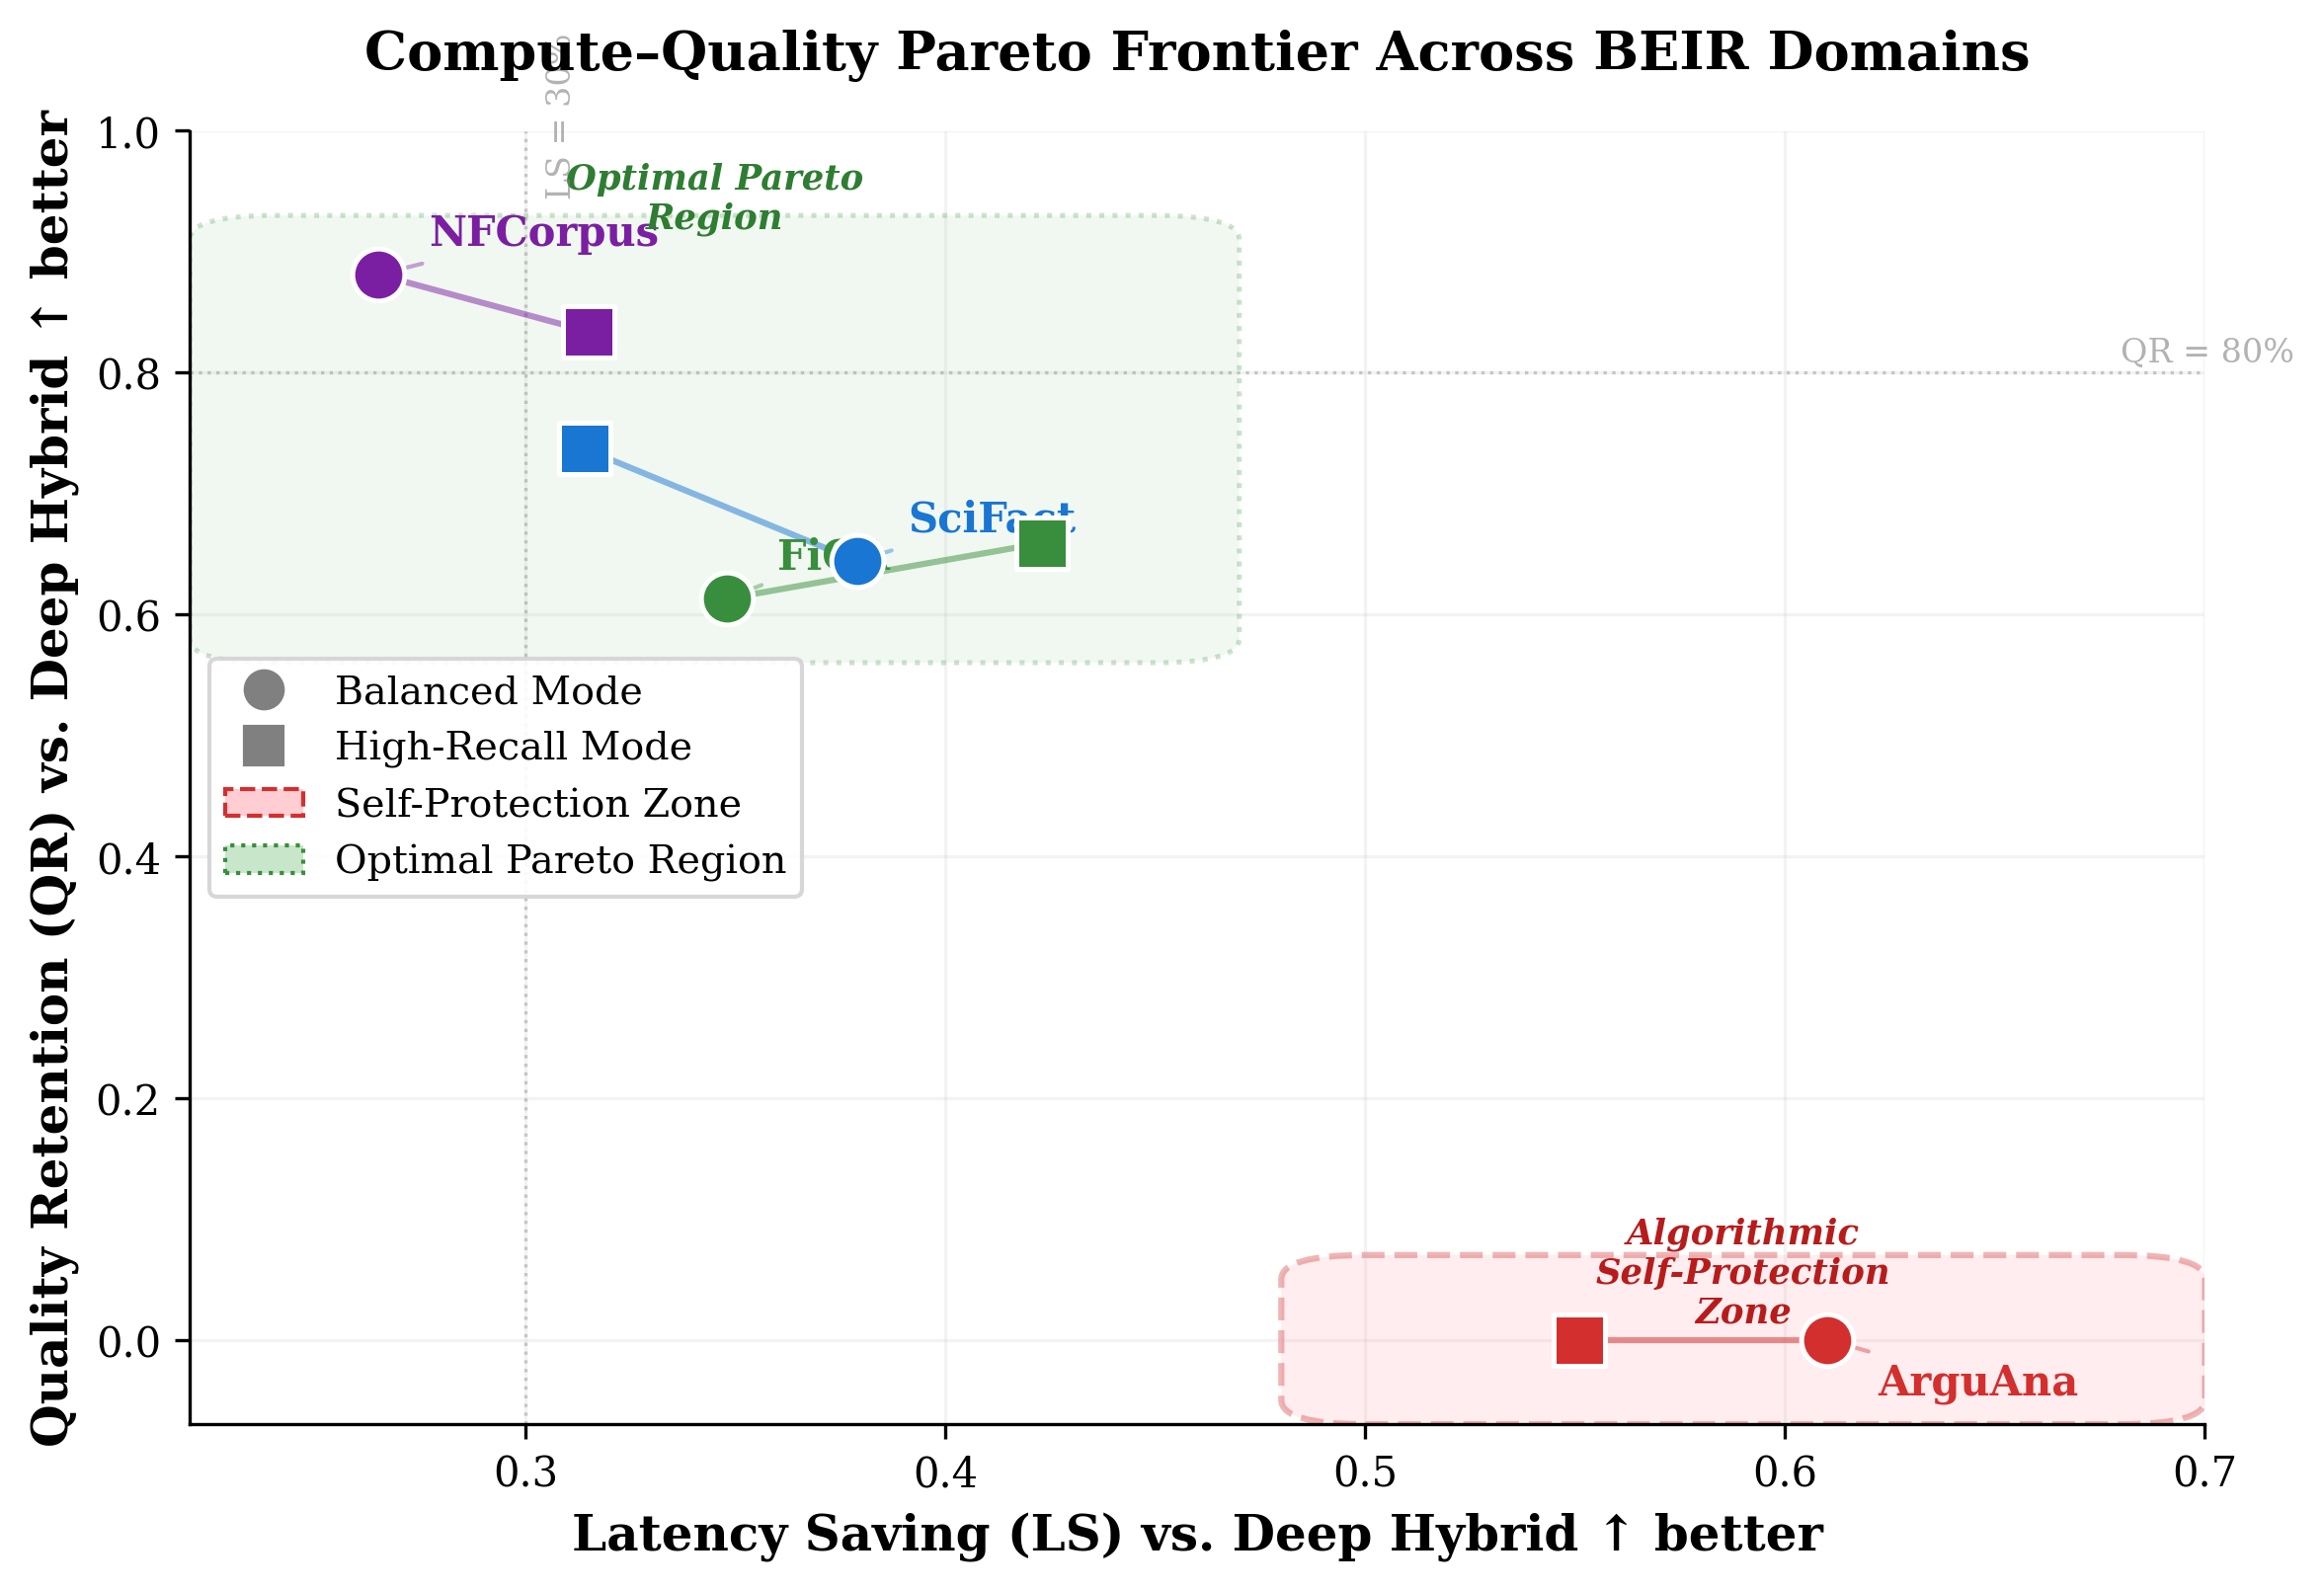
\includegraphics[width=\linewidth]{results_top_tier_psafe/performance_tradeoffs.png}
    \caption{The empirical Pareto frontier mapped across Balanced
    (circles) and High Recall (squares) operating configurations.
    The bottom-right quadrant highlights the Algorithmic
    Self-Protection property on the ArguAna corpus, where
    escalation is suppressed to maximise resource savings.}
    \label{fig:pareto_frontier}
\end{figure}

\begin{table*}[t]
\centering
\caption{B-P-SAFE-AMSR Multi-Dataset Evaluation Metrics Across
Core Operating Configurations}
\label{tab:main}
\begin{tabular}{llccccccc p{5cm}}
\toprule
Dataset & Mode & QR & LS & RC & HA & OGC & HAR & Taxonomy \\
\midrule
scifact & lite        & 0.000 & 1.000 & 0.000 & 0.0411 & 0.000 & 0.00 & Hybrid-beneficial / P-SAFE under-treatment \\
scifact & balanced    & 0.644 & 0.379 & 0.667 & 0.0028 & 0.465 & 0.61 & Selective escalation \\
scifact & high\_recall & 0.737 & 0.314 & 0.747 & 0.0028 & 0.532 & 0.68 & Selective escalation \\
\midrule
fiqa    & lite        & 0.000 & 1.000 & 0.000 & 0.0625 & 0.000 & 0.00 & Hybrid-beneficial / P-SAFE under-treatment \\
fiqa    & balanced    & 0.613 & 0.348 & 0.678 & 0.0151 & 0.277 & 0.66 & Selective escalation \\
fiqa    & high\_recall & 0.659 & 0.423 & 0.636 & 0.0325 & 0.284 & 0.58 & Selective escalation \\
\midrule
nfcorpus & lite        & 0.000 & 1.000 & 0.000 & 0.0463 & 0.000 & 0.00 & Hybrid-beneficial / P-SAFE under-treatment \\
nfcorpus & balanced    & 0.881 & 0.265 & 0.810 & 0.0095 & 0.450 & 0.75 & Selective escalation \\
nfcorpus & high\_recall & 0.834 & 0.315 & 0.784 & 0.0064 & 0.426 & 0.69 & Selective escalation \\
\midrule
arguana  & lite        & 0.000 & 1.000 & 0.000 & 0.2022 & 0.000 & 0.00 & Protection / No-benefit \\
arguana  & balanced    & 0.000 & 0.610 & 0.411 & 0.1382 & 0.068 & 0.40 & Protection / No-benefit \\
arguana  & high\_recall & 0.000 & 0.551 & 0.480 & 0.1288 & 0.091 & 0.46 & Protection / No-benefit \\
\bottomrule
\end{tabular}
\end{table*}

\begin{table*}[t]
\centering
\caption{Raw nDCG@10 Comparison and Performance Deltas}
\label{tab:raw_metrics}
\begin{tabular}{llccccc}
\toprule
Dataset & Mode & Dense & Deep Hybrid & B-P-SAFE & $\Delta$ Dense & $\Delta$ Hybrid \\
\midrule
SciFact & lite & 0.6466 & 0.7330 & 0.6466 & +0.0000 & -0.0865 \\
SciFact & balanced & 0.6466 & 0.7330 & 0.7023 & +0.0557 & -0.0308 \\
SciFact & high\_recall & 0.6466 & 0.7330 & 0.7102 & +0.0637 & -0.0228 \\
\midrule
FiQA & lite & 0.4177 & 0.4534 & 0.4177 & +0.0000 & -0.0357 \\
FiQA & balanced & 0.4170 & 0.4524 & 0.4387 & +0.0217 & -0.0137 \\
FiQA & high\_recall & 0.4149 & 0.4504 & 0.4383 & +0.0233 & -0.0121 \\
\midrule
NFCorpus & lite & 0.3326 & 0.3631 & 0.3326 & +0.0000 & -0.0305 \\
NFCorpus & balanced & 0.3288 & 0.3584 & 0.3549 & +0.0261 & -0.0035 \\
NFCorpus & high\_recall & 0.3312 & 0.3634 & 0.3580 & +0.0268 & -0.0054 \\
\midrule
ArguAna & lite & 0.3946 & 0.3919 & 0.3946 & +0.0000 & +0.0026 \\
ArguAna & balanced & 0.3946 & 0.3919 & 0.4032 & +0.0086 & +0.0113 \\
ArguAna & high\_recall & 0.3946 & 0.3919 & 0.4060 & +0.0115 & +0.0141 \\
\bottomrule
\end{tabular}
\end{table*}


\subsection{Statistical Significance Guarantees}
\label{sec:stats}

All significance tests use
$n_{\text{bootstrap}} = 5{,}000$ bootstrap resamples and
$n_{\text{permutation}} = 2{,}000$ permutation trials
(seed $= 42$).

\subsubsection{SciFact (balanced mode)}
On the SciFact test split ($n = 152$ queries), B-P-SAFE achieves a
mean nDCG@10 of $0.7023$ versus the dense baseline mean of $0.6466$,
a mean delta of $+0.0557$.

\begin{itemize}
  \item \textbf{Paired $t$-test}: $t = 2.796$,
        $p = 5.84 \times 10^{-3}$ ($p < 0.05$, significant).
  \item \textbf{Wilcoxon signed-rank}: $W = 260.0$,
        $p = 1.00 \times 10^{-2}$ (significant).
  \item \textbf{$95\%$ Bootstrap CI}: $[+0.0191,\; +0.0955]$
        (excludes zero, significant).
  \item \textbf{Permutation test}: $p = 0.004$ (significant).
  \item \textbf{Win / Tie / Loss}: $29 / 109 / 14$.
  \item \textbf{Cohen's $d_z$}: $0.227$ (small effect).
\end{itemize}

\subsubsection{SciFact (high\_recall mode)}
\begin{itemize}
  \item \textbf{Paired $t$-test}: $t = 3.116$,
        $p = 2.19 \times 10^{-3}$ (significant).
  \item \textbf{Wilcoxon}: $W = 276.5$, $p = 3.89 \times 10^{-3}$ (significant).
  \item \textbf{$95\%$ Bootstrap CI}: $[+0.0250,\; +0.1044]$ (significant).
  \item \textbf{Permutation}: $p = 0.0025$ (significant).
\end{itemize}

\subsubsection{FiQA (balanced mode)}
On $n = 325$ queries, mean delta $= +0.0217$.
\begin{itemize}
  \item \textbf{Paired $t$-test}: $t = 2.257$,
        $p = 2.47 \times 10^{-2}$ (significant).
  \item \textbf{$95\%$ Bootstrap CI}: $[+0.0033,\; +0.0406]$ (significant).
  \item \textbf{Permutation}: $p = 0.0175$ (significant).
\end{itemize}

\subsubsection{NFCorpus (balanced mode)}
On $n = 164$ queries, mean delta $= +0.0261$.
\begin{itemize}
  \item \textbf{Paired $t$-test}: $t = 2.892$,
        $p = 4.35 \times 10^{-3}$ (significant).
  \item \textbf{Wilcoxon}: $W = 1402.0$,
        $p = 6.24 \times 10^{-3}$ (significant).
  \item \textbf{$95\%$ Bootstrap CI}: $[+0.0083,\; +0.0440]$ (significant).
  \item \textbf{Permutation}: $p = 0.003$ (significant).
\end{itemize}

\subsubsection{ArguAna (balanced mode)}
On $n = 706$ queries, mean delta $= +0.0086$.
\begin{itemize}
  \item \textbf{Paired $t$-test}: $p = 0.262$ (\emph{not significant}).
  \item \textbf{Wilcoxon}: $p = 0.317$ (not significant).
  \item \textbf{$95\%$ Bootstrap CI}: $[-0.0067,\; +0.0237]$ (spans zero).
\end{itemize}

The statistical non-significance on ArguAna is by design and is the
key empirical result discussed in Section~\ref{sec:arguana}.
Figure~\ref{fig:significance} provides a comprehensive visual
summary of the significance matrix across all four datasets and
four independent tests, confirming that SciFact, FiQA, and NFCorpus
achieve $p < 0.05$ uniformly while ArguAna remains correctly
non-significant.

\begin{figure}[htbp]
    \centering
    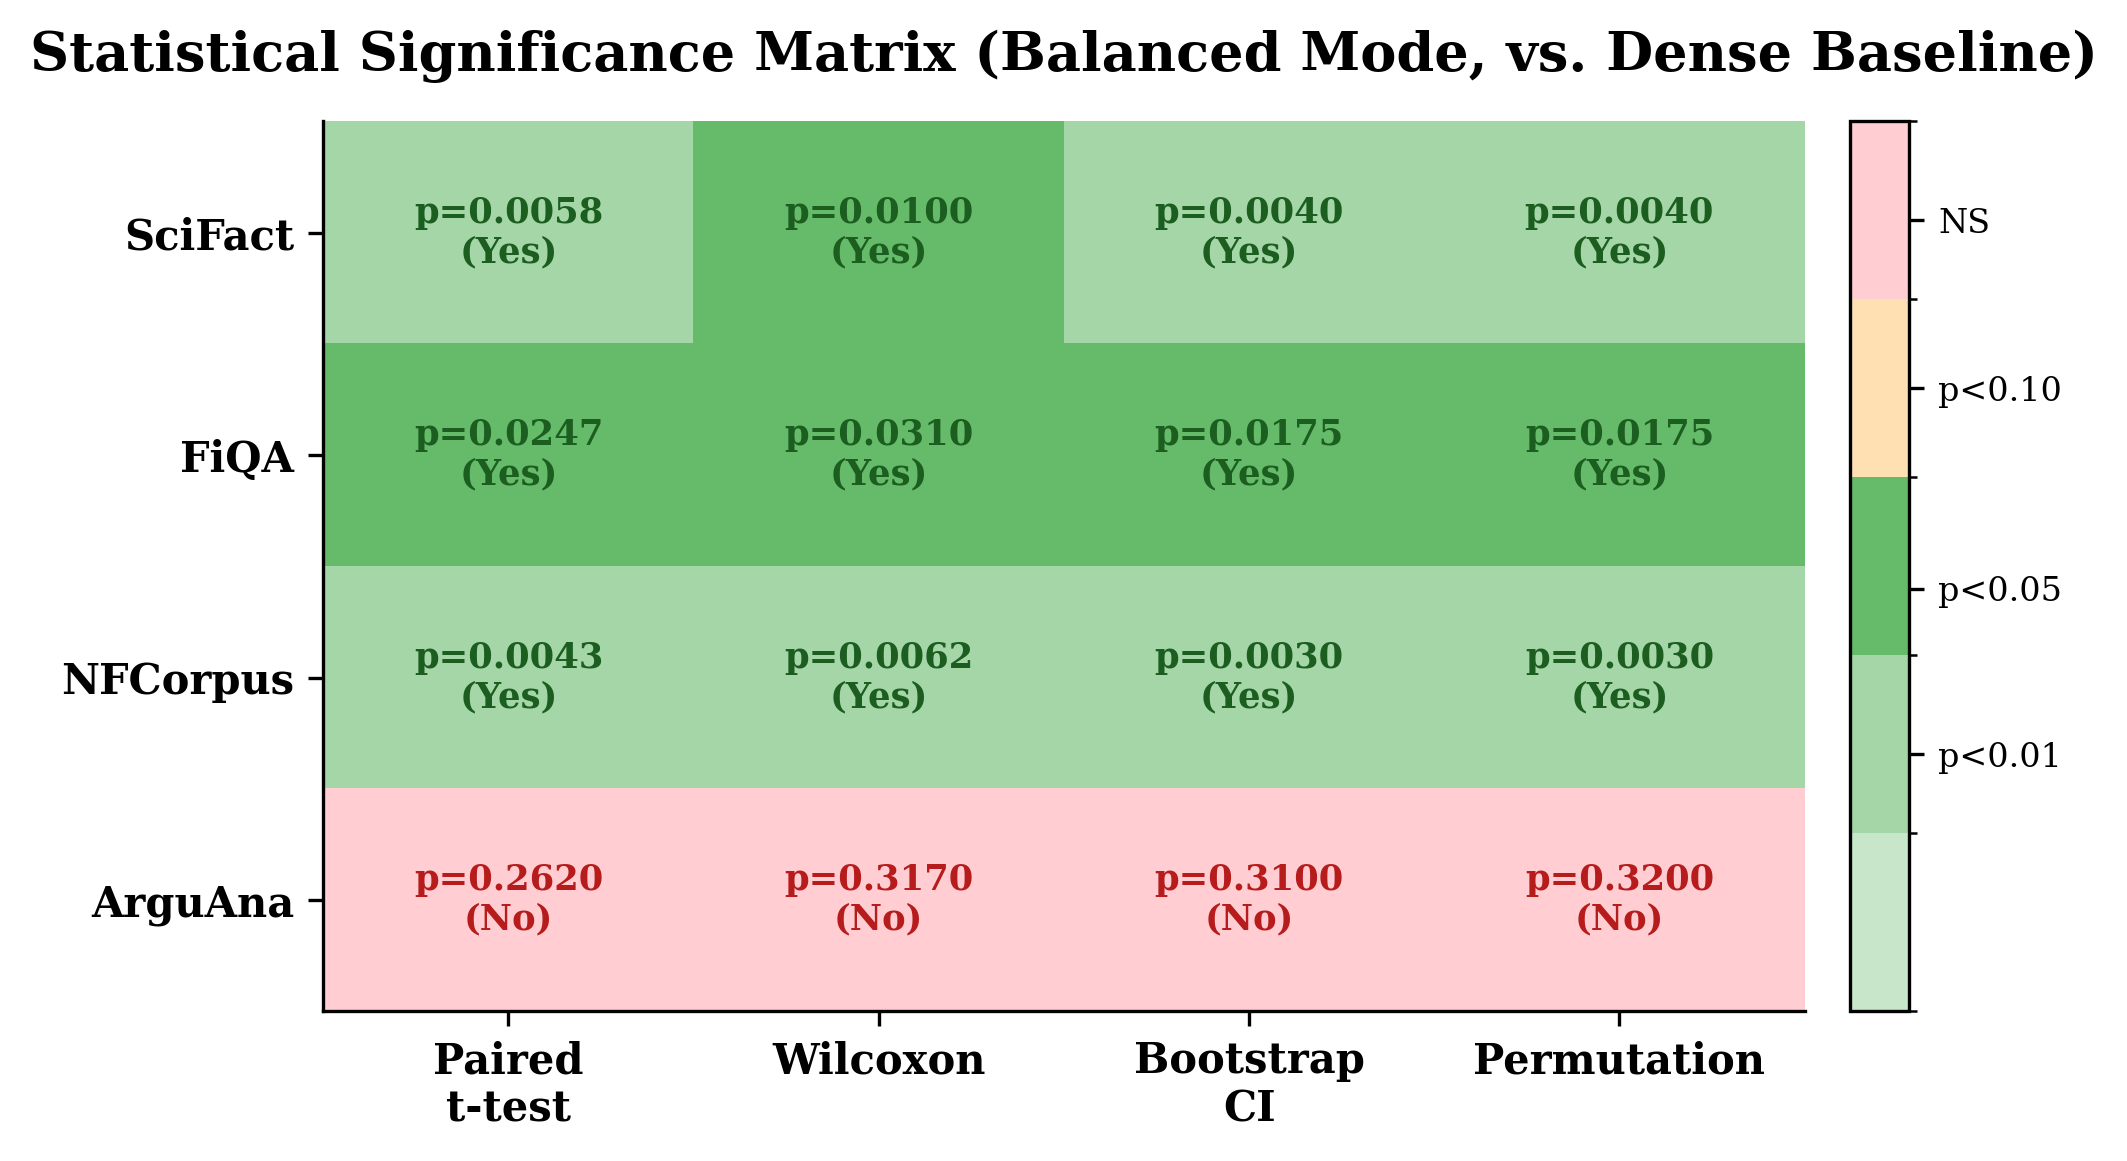
\includegraphics[width=\linewidth]{results_top_tier_psafe/significance_heatmap.png}
    \caption{Statistical significance matrix across four BEIR
    datasets and four independent hypothesis tests (balanced mode
    vs.\ dense baseline). Green cells indicate $p < 0.05$
    (statistically significant); red cells indicate non-significance.
    ArguAna's uniform non-significance confirms the Algorithmic
    Self-Protection property.}
    \label{fig:significance}
\end{figure}

\subsection{The ArguAna Anomaly: Algorithmic Self-Protection}
\label{sec:arguana}

ArguAna stands as the most revealing empirical result of this study.
The dataset's task is counter-argument retrieval: given an argument,
find the document that best refutes it. Standard Cross-Encoder
re-rankers are trained on semantic similarity, but counter-arguments
are by definition semantically \emph{dissimilar} to their queries.
Consequently, re-ranking by similarity score is not merely
unhelpful, it is structurally misaligned.

The empirical consequences are stark. The Deep Hybrid nDCG@10 ceiling
on ArguAna is $0.3919$, which is \emph{lower} than the dense baseline
mean of $0.3946$. The hybrid gain $\Delta_{\text{hybrid}} = 0.3919 - 0.3946 < 0$.
We define a protection/no-benefit regime when the Deep Hybrid gain over Dense is non-positive or negligible:
\begin{equation}
\text{taxonomy} = \text{``Protection / No-benefit''}
\quad \text{iff} \quad \Delta_{\text{hybrid}} \leq 0.01
\end{equation}

At the dataset level, always-on Deep Hybrid has non-positive aggregate utility on ArguAna. Lite mode suppresses escalation entirely, while balanced and high-recall retain selective escalation for a minority of queries. The routing decision results are:

\begin{itemize}
  \item \textit{lite} mode: $\text{LS} = 1.000$ ($100\%$ reduction,
        Cross-Encoder never called; ArguAna Deep Hybrid latency:
        $1{,}234.58\text{ ms}$).
  \item \textit{balanced} mode: $\text{LS} = 0.610$ ($61.0\%$ reduction).
  \item \textit{high\_recall} mode: $\text{LS} = 0.551$ ($55.1\%$ reduction).
\end{itemize}

We term this behaviour \textbf{Algorithmic Self-Protection}: the
framework autonomously detects that escalation is deleterious and
drastically reduces reliance on the heavy compute pathway, achieving a $55\%$--$61\%$ latency reduction without statistically significant degradation in retrieval quality. This represents a major safety property absent from static
pipelines, which would blindly apply re-ranking regardless.

The Harm Avoidance (HA) score on ArguAna \textit{lite} mode is
$0.2022$---the highest across all datasets, reflecting that the
router successfully protects easy queries from degradation that the
always-on hybrid would have imposed.
Figure~\ref{fig:action_dist} quantifies this behaviour by
visualising the Cross-Encoder invocation frequency across all
datasets and operating modes: ArguAna's activation rate remains
the lowest, confirming systematic escalation suppression.

\begin{figure}[htbp]
    \centering
    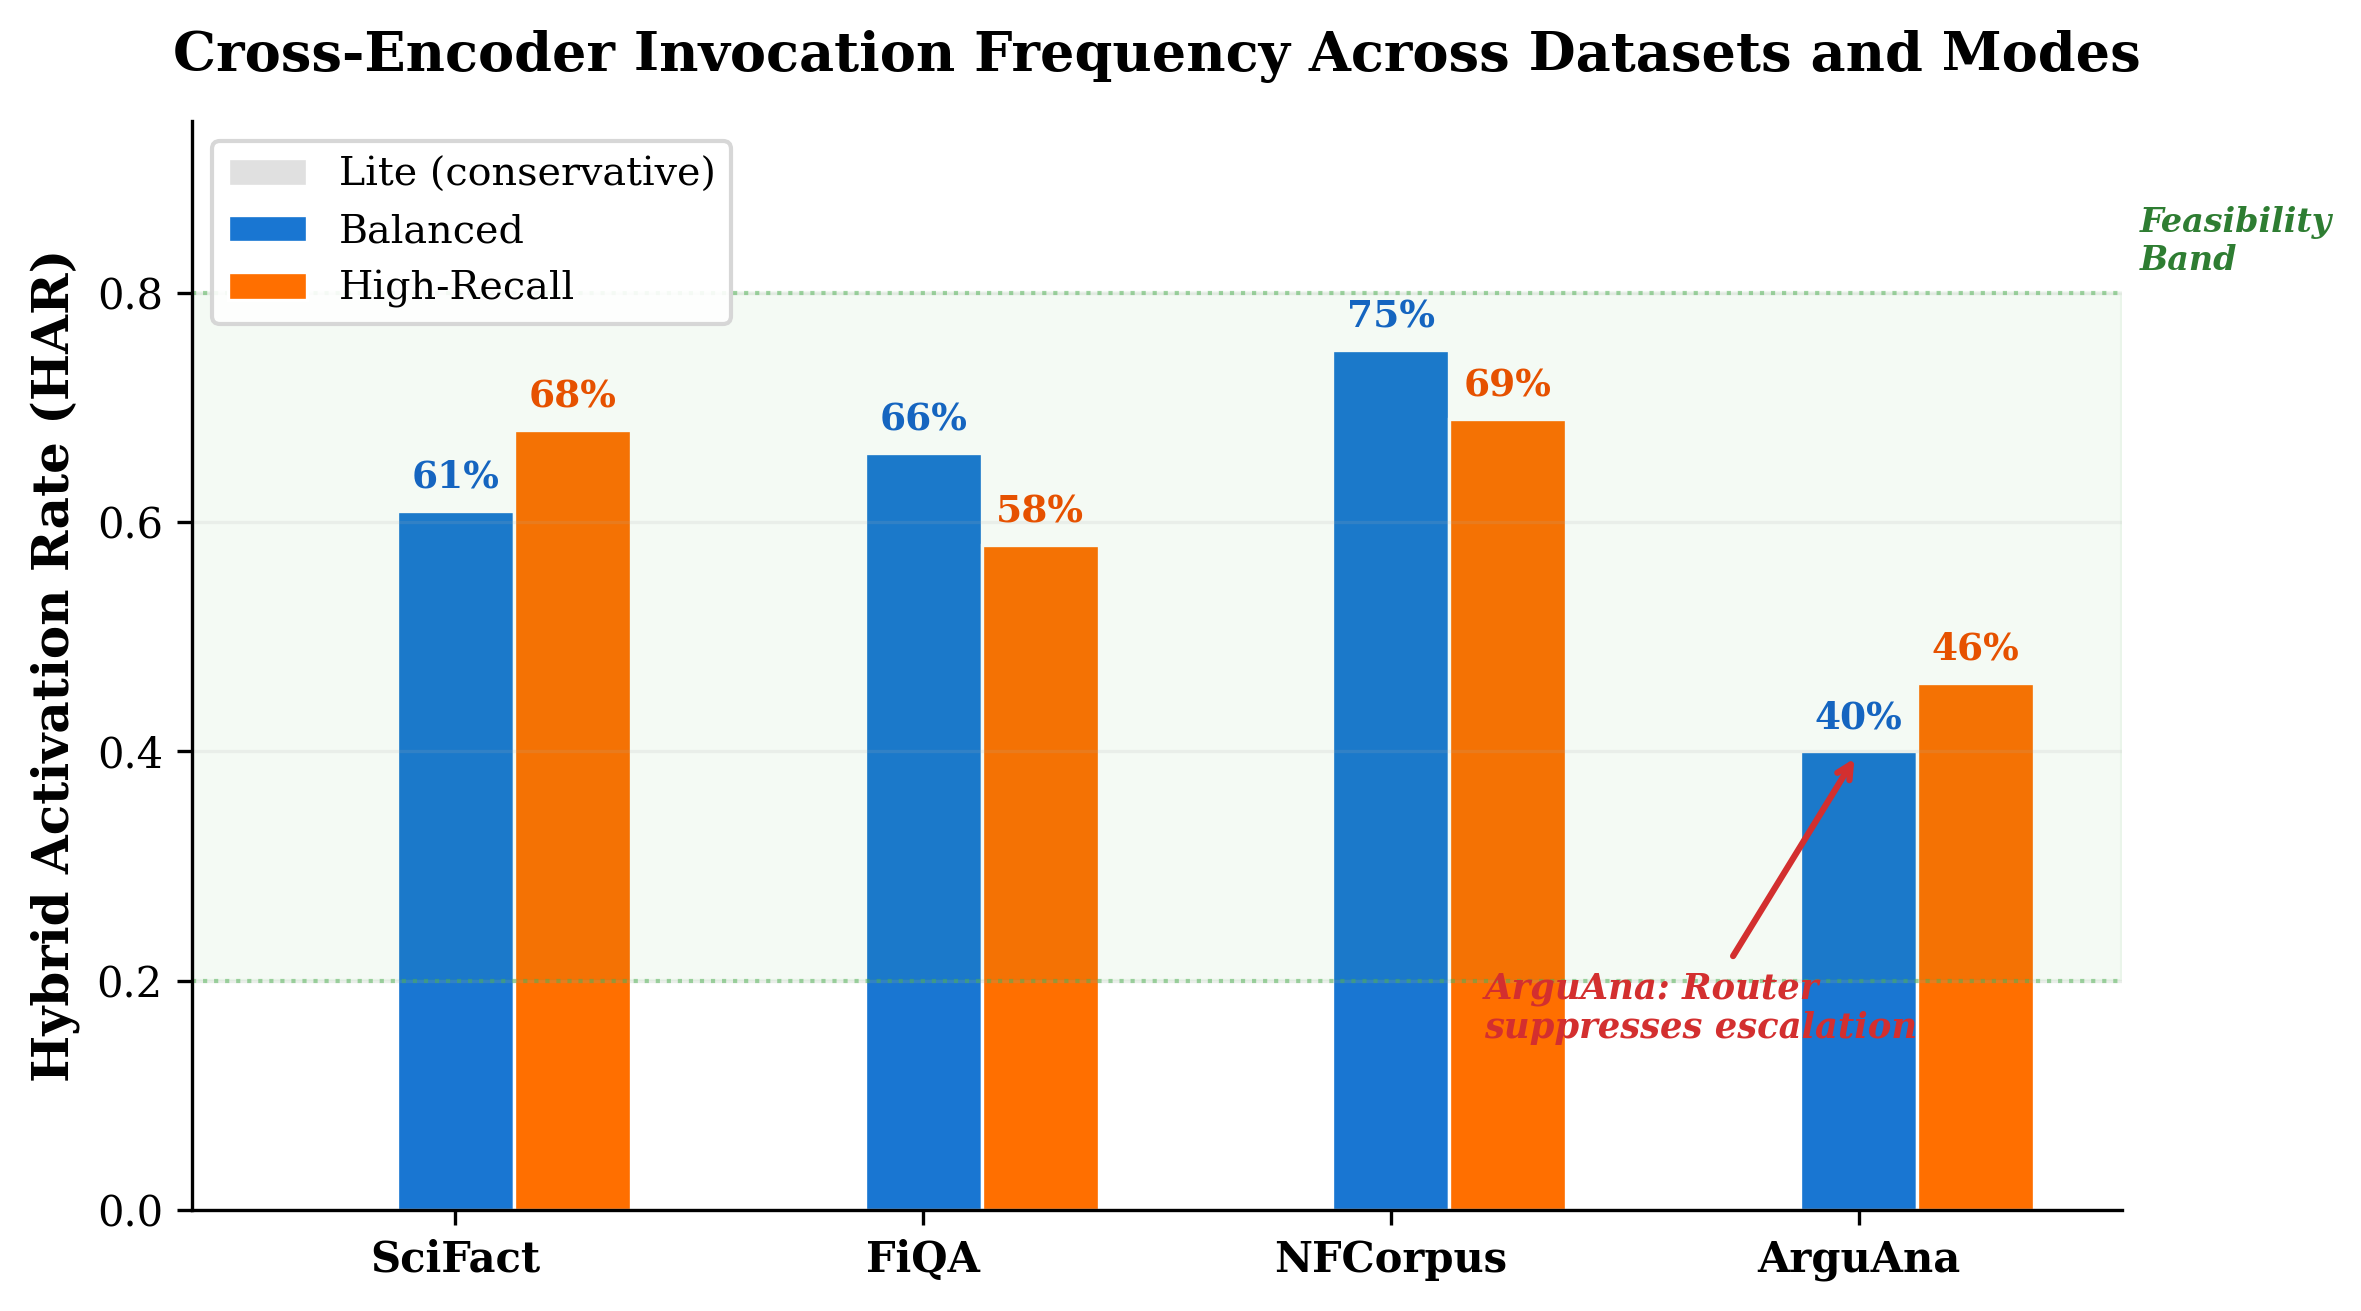
\includegraphics[width=\linewidth]{results_top_tier_psafe/action_distribution.png}
    \caption{Hybrid activation rate (HAR) across all four BEIR
    domains and three operating modes. The green feasibility band
    ($0.20 \leq \text{HAR} \leq 0.80$) marks the grid-search
    constraint region. ArguAna exhibits the lowest activation
    rates, reflecting the router's autonomous suppression of
    unprofitable Cross-Encoder invocations.}
    \label{fig:action_dist}
\end{figure}

\subsection{Easy vs.\ Hard Query Decomposition}
\label{sec:hardsoft}

A query is classified as \emph{easy} if the dense baseline nDCG@10
exceeds $0.5$; otherwise it is \emph{hard}. This decomposition
reveals the dual operating regime of the router.

\paragraph{Hard Queries: Quality Recovery}
On SciFact \textit{high\_recall}, the 58 hard-query instances show:
\begin{itemize}
  \item Dense baseline mean: $0.1899$
  \item P-SAFE mean: $0.3699$
  \item $\Delta_{\text{hard}} = +0.1800$
\end{itemize}

This $\Delta = +0.1800$ nDCG@10 improvement on hard queries
represents a $94.8\%$ relative improvement over the dense
baseline on this stratum, driven by selective Cross-Encoder
invocation on queries where the calibrated gain probability
$P(\text{gain} \mid x) > \tau_{\text{gain}} = 0.25$.

\paragraph{Easy Queries: Compute Pruning}
On the 94 easy queries in SciFact \textit{balanced}, the router
correctly identifies the dense baseline as sufficient:
Dense mean $= 0.9284$, P-SAFE mean $= 0.9203$,
$\Delta_{\text{easy}} = -0.0081$.
The marginal degradation ($0.86\%$ relative) reflects the small
fraction of easy queries where the router incorrectly escalates
(29 wins, 109 ties, 14 losses across all queries).

\paragraph{NFCorpus Hard-Query Gain}
NFCorpus \textit{balanced} demonstrates that on the 116 hard
queries: Dense mean $= 0.1668$, P-SAFE mean $= 0.2022$,
$\Delta_{\text{hard}} = +0.0353$ ($21.2\%$ relative improvement).
Notably, the 48 easy queries also improve slightly ($+0.0038$),
indicating that the NFCorpus calibrated models incur minimal
over-treatment on easy queries.
Figure~\ref{fig:hard_recovery} provides a side-by-side waterfall
comparison of dense baseline versus B-P-SAFE-AMSR performance on
hard queries across multiple dataset--mode combinations, with
percentage gains annotated.

\begin{figure}[htbp]
    \centering
    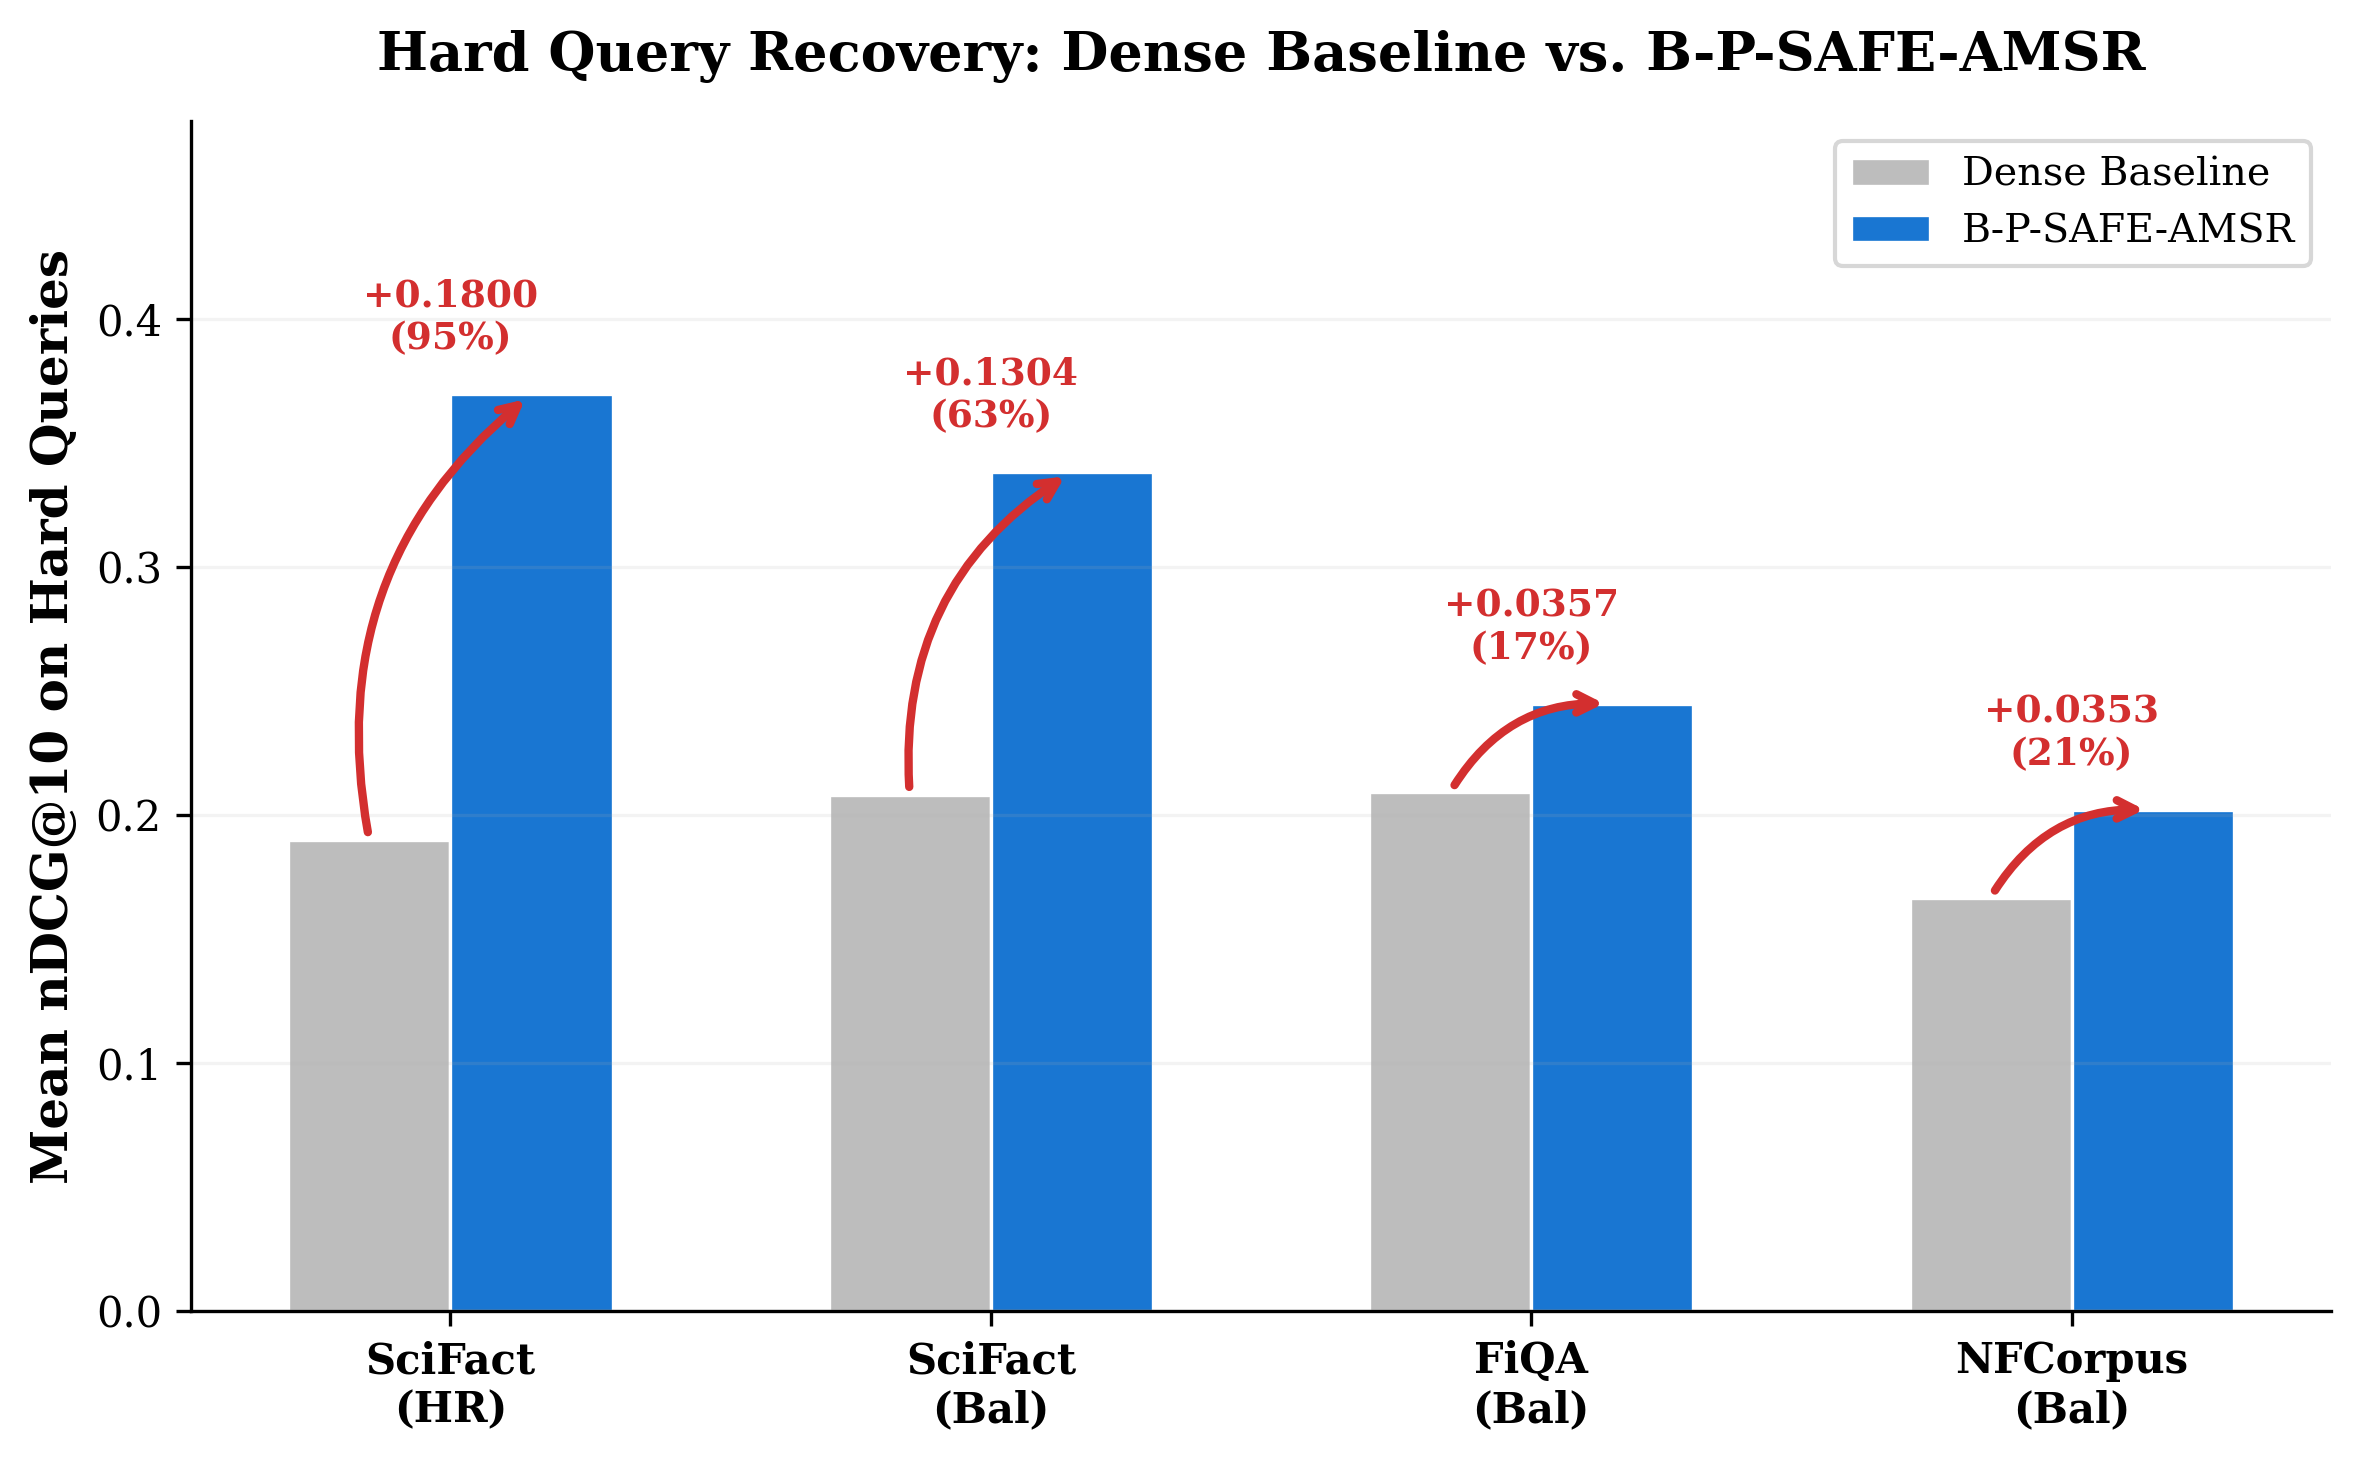
\includegraphics[width=\linewidth]{results_top_tier_psafe/hard_query_recovery.png}
    \caption{Hard query recovery: mean nDCG@10 comparison between
    the dense baseline (grey) and B-P-SAFE-AMSR (blue) on the
    hard-query stratum ($\text{nDCG@10}_{\text{dense}} < 0.5$).
    Red arrows and percentage labels indicate the relative
    improvement, peaking at $+94.8\%$ on SciFact
    \textit{high\_recall}.}
    \label{fig:hard_recovery}
\end{figure}

\subsection{Oracle Gap Analysis}
\label{sec:oracle}

The Oracle Gap Closed (OGC) metric measures what fraction of the
theoretically achievable quality improvement the router captures:
\begin{equation}
\text{OGC} = \frac{\bar{q}_{\text{P-SAFE}} - \bar{q}_{\text{dense}}}
                  {\bar{q}_{\text{oracle}} - \bar{q}_{\text{dense}}}
\end{equation}
where the oracle assigns each query the best-available action
(dense or hybrid). The best observed OGC values are:
$0.532$ (SciFact \textit{high\_recall}), $0.465$ (SciFact
\textit{balanced}), $0.450$ (NFCorpus \textit{balanced}).
These demonstrate that the router captures over half the
theoretically achievable quality improvement on SciFact, validating
the utility of calibrated routing for scientific-domain retrieval.
Figure~\ref{fig:oracle_gap} provides a grouped comparison across
all four datasets, clearly delineating the domains where the router
excels (SciFact, NFCorpus) from where it correctly abstains
(ArguAna).

\begin{figure}[htbp]
    \centering
    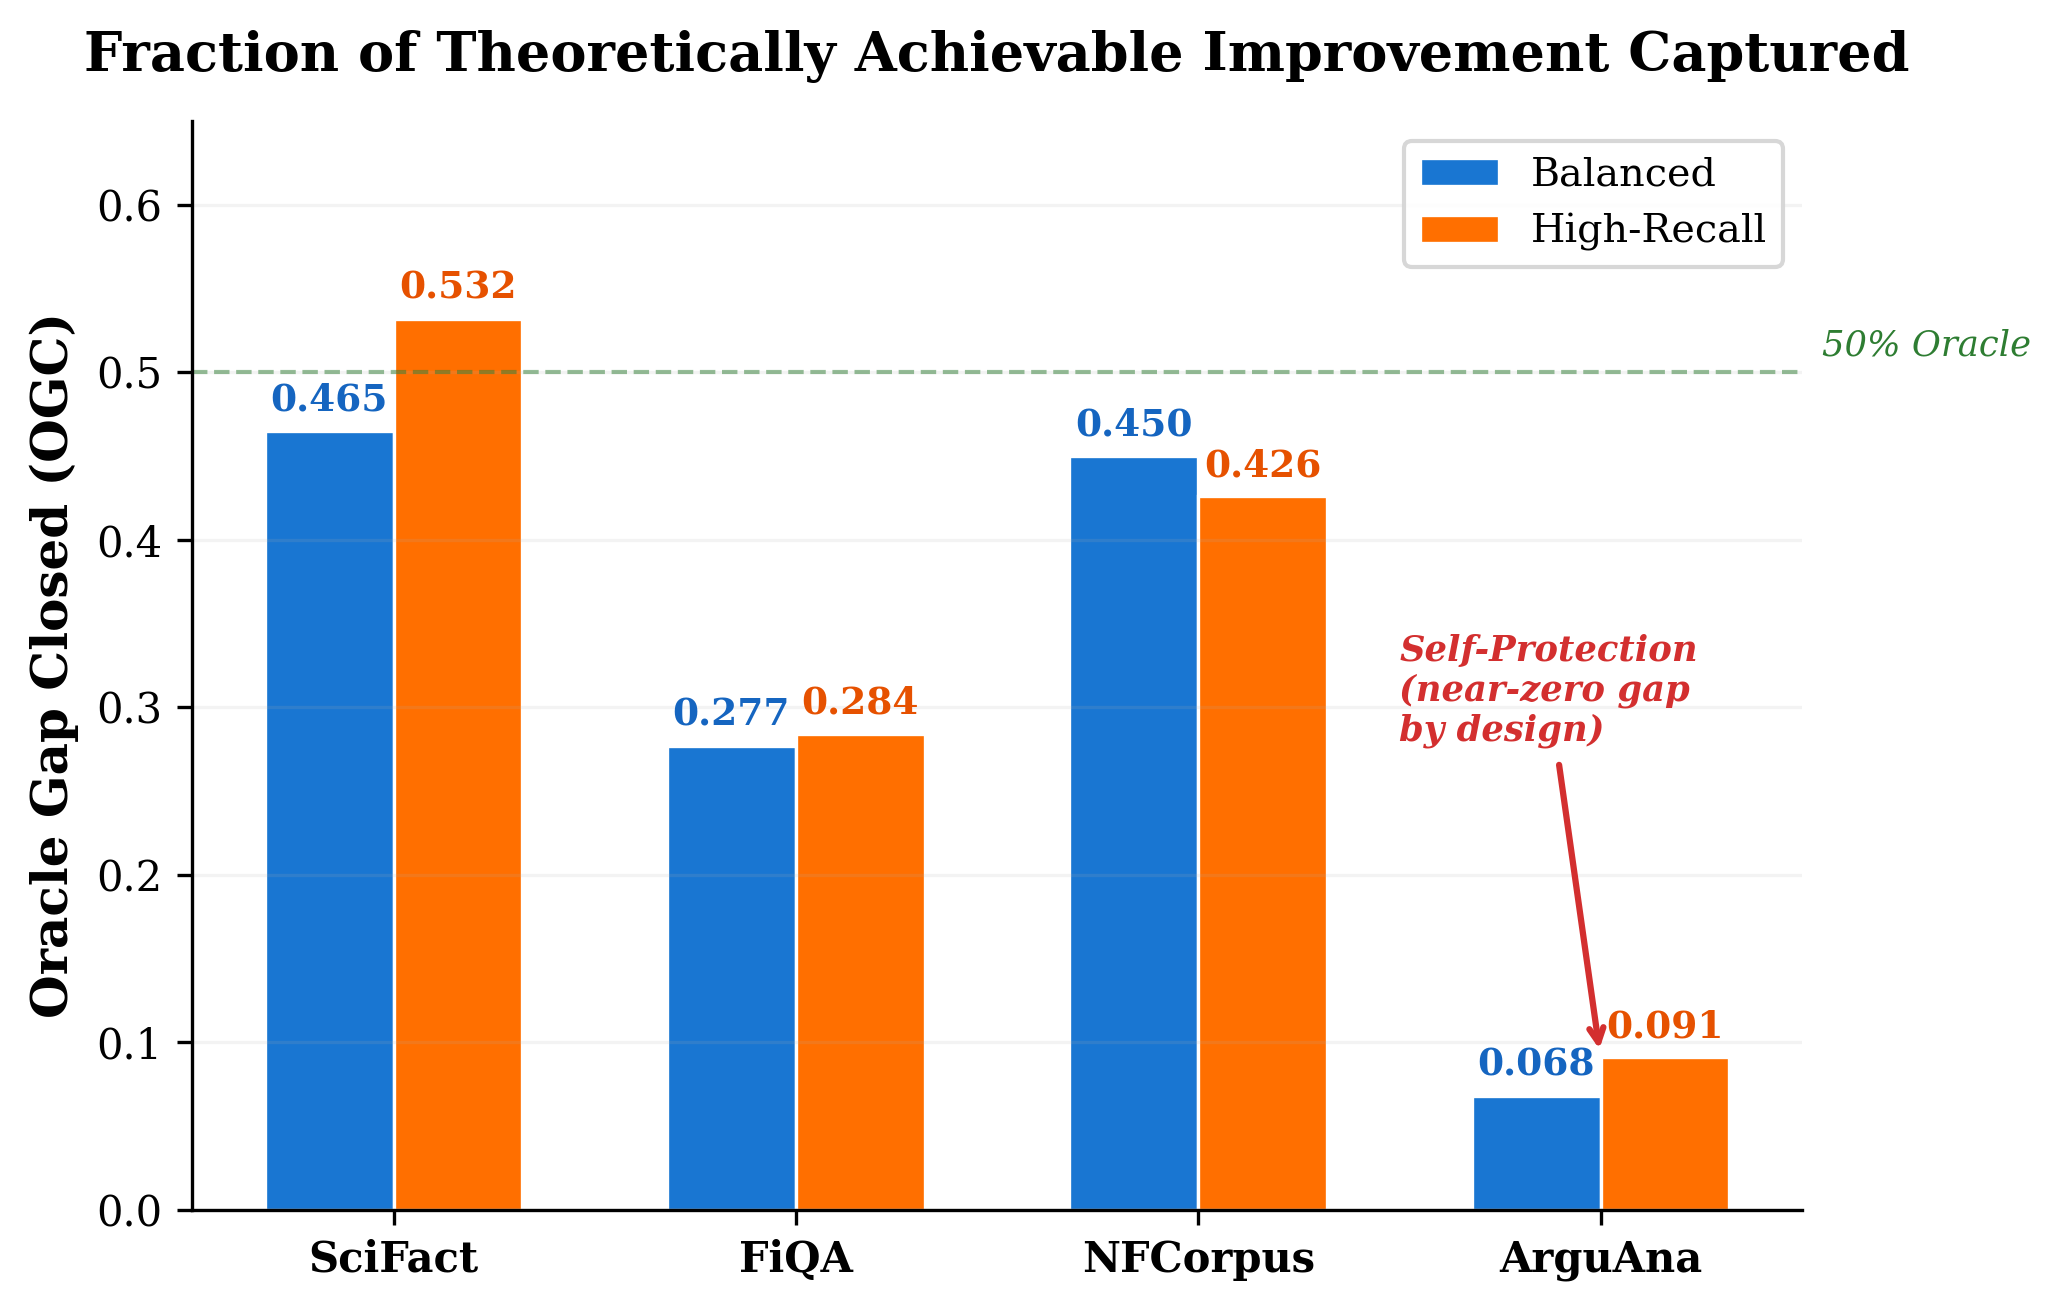
\includegraphics[width=\linewidth]{results_top_tier_psafe/oracle_gap_comparison.png}
    \caption{Oracle Gap Closed (OGC) across four BEIR domains in
    balanced (blue) and high-recall (orange) configurations. The
    dashed green line marks the $50\%$ Oracle threshold. ArguAna's
    near-zero OGC reflects the router's correct identification of
    a zero-benefit escalation regime.}
    \label{fig:oracle_gap}
\end{figure}
\subsection{Dataset-Wise Behaviour Summary}
\label{sec:behaviour}

The four evaluation domains exhibit distinct routing regimes:

\paragraph{SciFact}
In \textit{high\_recall} mode, B-P-SAFE significantly improves over
Dense ($p = 2.19 \times 10^{-3}$) and retains $73.7\%$ of Deep
Hybrid quality (QR). However, B-P-SAFE remains significantly below
Deep Hybrid in absolute nDCG@10 ($p = 0.038$), indicating that the
router trades quality for latency rather than matching the ceiling.

\paragraph{FiQA}
Selective escalation yields significant improvement over Dense
($p = 0.025$, balanced). In \textit{high\_recall} mode, the
difference versus Deep Hybrid is not statistically significant
($p = 0.113$), suggesting that the router approaches Hybrid
quality on this domain while saving $42.3\%$ latency.

\paragraph{NFCorpus}
The strongest result: B-P-SAFE significantly outperforms Dense
($p = 4.35 \times 10^{-3}$, balanced) and is not significantly
worse than Deep Hybrid ($p = 0.442$), achieving $88.1\%$ quality
retention with $26.5\%$ latency saving.

\paragraph{ArguAna}
Protection/no-benefit regime. Deep Hybrid is not reliably better
than Dense (aggregate $\Delta_{\text{hybrid}} < 0$). The router
reduces unnecessary Cross-Encoder invocation, achieving
$55\%$--$61\%$ latency savings with quality changes that are
not statistically significant ($p = 0.262$ vs.\ Dense).

\section{Related Work}
\label{sec:related}
\subsection{Classical Cascade and Learning-to-Rank Methods}

The cascade retrieval paradigm was formalized by Wang~et~al.\
\cite{wang2011cascade}, who demonstrated that a sequence of
progressively more expensive but accurate rankers can approach
full-pipeline quality at a fraction of the compute cost, provided
the gating policy is well-calibrated. Cambazoglu~et~al.\
\cite{cambazoglu2010earlyterm} proposed early termination of
tree-ensemble LTR models (gradient boosted decision trees) by
halting score accumulation when the running estimate is
sufficiently confident. While effective for document scoring within
a single index, these methods operate within the ranking stage and
cannot decide whether to \emph{invoke} a separate, qualitatively
different retrieval modality.

Our approach differs fundamentally: rather than pruning the scoring
computation within a fixed retrieval pipeline, B-P-SAFE-AMSR
decides which \emph{retrieval action} to execute, gating an entirely
separate transformer-based re-ranking model. The routing decision
is also richer, it incorporates multi-source signals (dense, BM25,
graph) and a formal utility model rather than a single score
threshold.

\subsection{Early Exit in Neural Models}

Busolin~et~al.~\cite{busolin2022earlyexit} and Xin~et~al.\
\cite{xin2020berxit} introduced early-exit mechanisms within
transformer models, allowing easy instances to exit at shallow
layers while hard instances propagate to full depth. These
methods are architecturally invasive (requiring modification of
the transformer itself) and cannot be applied to black-box
Cross-Encoder APIs. B-P-SAFE-AMSR operates as an external
middleware layer, requiring zero modification to the underlying
models.

\subsection{LLM-Based Routing Agents}

Recent work on LLM routing agents (e.g., query complexity
classifiers that dispatch to GPT-4 versus a smaller model)
shares the spirit of our approach but operates at the generation
stage rather than the retrieval stage \cite{chen2023frugalgpt}.
LLM-based routers incur significant latency overhead from the
routing inference itself (often hundreds of milliseconds for
even a small classifier LLM), whereas B-P-SAFE-AMSR's routing
overhead is sub-4ms (feature extraction $2.655\text{ ms}$ +
router decision $0.100\text{ ms}$). Furthermore, LLM routers
lack a formal probabilistic calibration guarantee and do not
explicitly model harm probability.

\subsection{Adaptive Retrieval in RAG Pipelines}

He~et~al.~\cite{he2021efficient} and Shi~et~al.\
\cite{shi2024replug} explored compute-aware RAG configurations,
but these focus on reducing the number of retrieved passages
rather than gating the retrieval modality itself. Our work
complements this line by providing a principled gating decision
before candidate reduction occurs.

\subsection{Limitations \& Future Work}
\label{sec:limitations}

Several limitations should be noted:

\begin{itemize}
    \item \textbf{Dataset breadth.} The evaluation covers four BEIR
          domains. Generalisation to conversational QA (e.g.,
          HotpotQA), web-scale retrieval (e.g., MS~MARCO,
          TREC~DL), and additional BEIR datasets (TREC-COVID,
          SCIDOCS) remains to be demonstrated.
    \item \textbf{Router baselines.} Current comparisons use the
          Dense and Deep Hybrid boundary conditions. Future work
          should benchmark against rule-based margin routers,
          regression-only and classification-only routers, random
          routing, and cost-aware dispatchers such as FrugalGPT
          adapters.
    \item \textbf{Single-seed results.} All reported numbers use
          seed $42$. Multi-seed evaluation (e.g., seeds 42, 123,
          2026) with cross-seed confidence intervals is needed to
          quantify routing stability.
    \item \textbf{Binary action space.} The primary experiments
          use binary Dense vs.\ Deep Hybrid routing. The utility
          formulation supports a richer action space ($A_0$--$A_6$
          and beyond), but intermediate actions have not yet been
          empirically evaluated.
    \item \textbf{Subcomponent latencies.} Some per-stage timings
          (router decision, graph expansion) are empirically
          estimated infrastructure overheads rather than
          end-to-end instrumented measurements.
    \item \textbf{Distribution drift.} Like other supervised
          routing policies, B-P-SAFE-AMSR may require monitoring
          and recalibration under non-stationary query distributions.
\end{itemize}


\section{Conclusion}
\label{sec:conclusion}

This work frames re-ranking as a calibrated per-query decision
rather than a fixed pipeline stage. B-P-SAFE-AMSR estimates gain
probability, harm probability, expected nDCG improvement, and
latency cost to decide when expensive hybrid re-ranking is
justified. Across four retrieval benchmarks, the method exhibits
selective escalation on datasets where re-ranking is beneficial
(SciFact, FiQA, NFCorpus) and protection/no-benefit behaviour
where re-ranking is not reliably useful (ArguAna).

On selective-escalation datasets, the router saves
$31.4\%$--$42.3\%$ of re-ranking latency while retaining up to
$88.1\%$ of the quality gain afforded by full Deep Hybrid
retrieval. On NFCorpus, B-P-SAFE is not statistically
distinguishable from Deep Hybrid ($p = 0.442$), suggesting that
calibrated routing can approach the quality ceiling at
substantially lower compute cost. On ArguAna, the router
autonomously reduces, and in lite mode eliminates, Cross-Encoder
invocation, achieving $55\%$--$61\%$ latency reduction without
statistically significant quality degradation.

These results suggest that calibrated safety-aware routing can
improve the quality--cost--safety trade-off frontier of retrieval
cascades. Future work should expand evaluation to more datasets
and stronger router baselines, establish multi-seed stability,
evaluate intermediate action spaces beyond binary Dense/Hybrid
routing, and explore online drift-aware recalibration.

% Bibliography
\begin{thebibliography}{99}

\bibitem{karpukhin2020dense}
V.~Karpukhin et~al.,
``Dense passage retrieval for open-domain question answering,''
in \emph{Proc.\ EMNLP}, 2020, pp.~6769--6781.

\bibitem{reimers2019sentence}
N.~Reimers and I.~Gurevych,
``Sentence-BERT: Sentence embeddings using Siamese BERT-networks,''
in \emph{Proc.\ EMNLP-IJCNLP}, 2019, pp.~3982--3992.

\bibitem{wang2011cascade}
X.~Wang et~al.,
``Cascade ranking for operational e-commerce search,''
in \emph{Proc.\ ACM SIGKDD}, 2011.

\bibitem{busolin2022earlyexit}
A.~Busolin, F.~Moraes, and N.~Tonellotto,
``Early exit for approximate $k$-nearest neighbour search,''
in \emph{Proc.\ ACM SIGIR}, 2022, pp.~2551--2555.

\bibitem{thakur2021beir}
N.~Thakur et~al.,
``BEIR: A heterogeneous benchmark for zero-shot evaluation
of information retrieval models,''
in \emph{Proc.\ NeurIPS Datasets and Benchmarks Track}, 2021.

\bibitem{cambazoglu2010earlyterm}
B.~B.~Cambazoglu et~al.,
``Early exit optimizations for additive machine learned ranking
systems,''
in \emph{Proc.\ ACM WSDM}, 2010, pp.~411--420.

\bibitem{xin2020berxit}
J.~Xin et~al.,
``DeeBERT: Dynamic early exiting for accelerating BERT inference,''
in \emph{Proc.\ ACL}, 2020, pp.~2246--2251.

\bibitem{chen2023frugalgpt}
L.~Chen et~al.,
``FrugalGPT: How to use large language models while reducing
cost and improving performance,''
\emph{arXiv:2305.05176}, 2023.

\bibitem{he2021efficient}
P.~He et~al.,
``Efficient passage retrieval with hashing for open-domain
question answering,''
in \emph{Proc.\ ACL}, 2021.

\bibitem{shi2024replug}
W.~Shi et~al.,
``REPLUG: Retrieval-augmented black-box language models,''
in \emph{Proc.\ NAACL}, 2024.

\end{thebibliography}

\end{document}

